% !TEX root = ./document.tex

\documentclass[11pt]{article}

\usepackage{mystyle}
\usepackage{myvars}

%-----------------------------

\begin{document}

  \maketitle

  %-----------------------------
  %	TEXT
  %-----------------------------


  \section{Descripción del conjunto de datos}
  \label{sec:description}

    \paragraph{}
    El conjunto de datos sobre el cual se va a realizar el análisis de la varianza se refiere a una serie de mediciones sobre el número de pulgones por planta de trigo. El experimento fue realizado recogiendo $40$ plantas (muestras aleatorias que supondremos independientes) de trigo, durante un periodo de $6$ semanas.

    \paragraph{}
    Para la realización de este análisis se ha utilizado la plataforma SAS \cite{sas}, en concreto la \emph{University Edition}. En este caso, el conjunto de datos ha sido suministrado en forma de fragmento de código, el cual se incluye en la figura \ref{code:sas_1}. El conjunto de datos sigue una estructura tabular de $240$ filas (referidas a cada observación) y $3$ columnas (referidas a la \texttt{semana}, identificador de \texttt{muestra} en esa semana y \texttt{recuento} de pulgones en dicha observación) tal y como se muestra en la figura \ref{img:pulgones-print}. El código \emph{SAS} utilizado en este caso se muestra en la figura \ref{code:sas_2}.

    \begin{figure}[h]
      \centering
      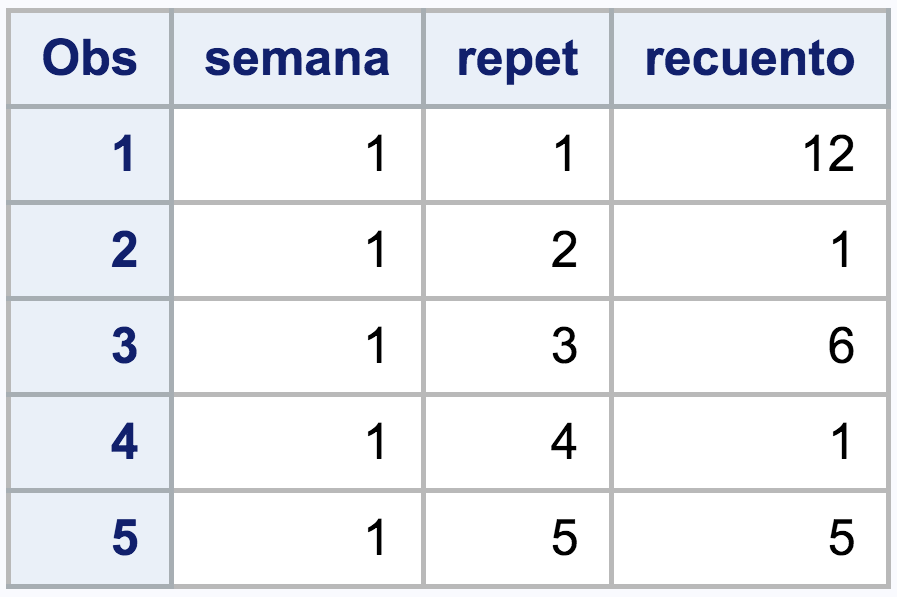
\includegraphics[width=.4\textwidth]{pulgones-print}
      \caption{Visión preliminar del conjunto de datos \texttt{pulgones}}
      \label{img:pulgones-print}
    \end{figure}

  \section{Cuestiones}
  \label{sec:questions}

    \paragraph{}
    El objetivo general del estudio es el siguiente: \textbf{\say{Se trata de analizar si existen diferencias en el número de pulgones por planta entre las diferentes semanas}}, para lo cual se proponen una seria de sub-objetivos que se tratarán de responder en las siguientes secciones.

    \subsection{?`Es adecuado utilizar un modelo de un factor para ello? Haz un análisis descriptivo de los datos por semanas y valora las hipótesis que se asumen en el modelo.}
    \label{sec:e1}

      \paragraph{}
      Para poder responder a la pregunta sobre si es adecuado utilizar un modelo de un factor para la comparación del número de pulgones por planta entre las distintas semananas, es necesario plantearse cómo han sido recogidas las observaciones, así como estudiar la distribución de la variable respuesta (\texttt{recuento} en este caso)

      \paragraph{}
      En el primer caso, se presupone que las $40$ observaciones referidas a cada semana han sido elegidas siguiendo algún procedimiento aleatorio. Por tanto, asumiremos como válida la hipótesis de independencia de las observaciones para la realización del análisis de un factor.

      \paragraph{}
      En cuanto a la hipótesis de normalidad, es decir, el estudio acerca de que los valores de la variable recuento siguen  una distribución aproximadamente normal, se ha realizado un estudio descriptivo sobre los mismos. Para dicha tarea se ha utilizado el fragmento de código incluido en la figura \ref{code:sas_3}. A partir de esta sentencia se han obtenido los resultados mostrados en la tabla de las figuras \ref{}, así como los \emph{Histogramas} incluidos en las figuras \ref{fig:histogram-plot-1-2}, \ref{fig:histogram-plot-3-4} y \ref{fig:histogram-plot-5-6} y los \emph{Gráficos de Normalidad} incluidos en las figuras \ref{fig:normal-plot-1-2}, \ref{fig:normal-plot-3-4} y \ref{fig:normal-plot-5-6}.

      \paragraph{}
      Tras el análisis de los mismos podemos empezar a sospechar acerca de una cierta falta de normalidad en los datos, concretamente en los referidos a las de la categoria \texttt{semana} $2$ y $3$. Esto se ve reflejado en los distintos valores de los tests de normalidad, así como en la apariencia de los histogramas y la marcada desviación respecto de la recta de la distirbución normal en los diagramas de \emph{cuantil-cuantil} respecto de la normal

      \begin{figure}
        \centering
        \begin{minipage}{.49\textwidth}
          \centering
          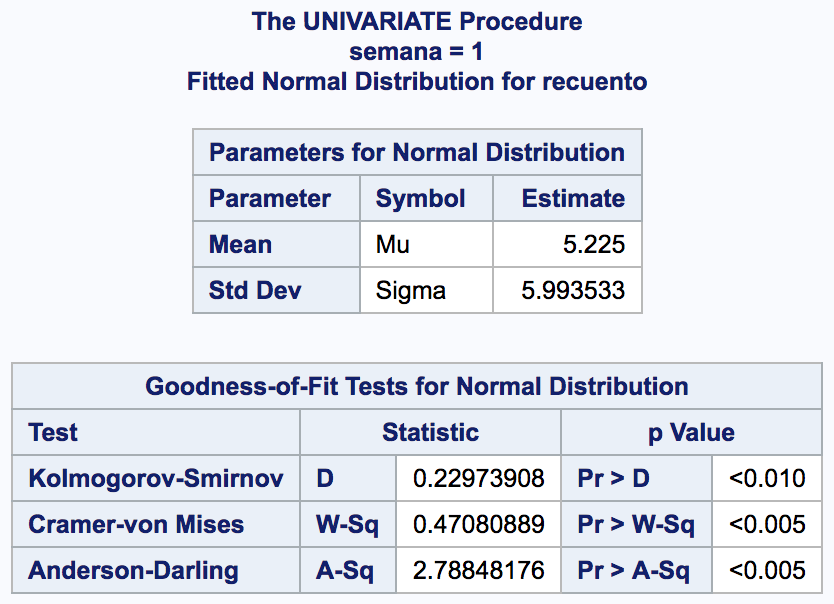
\includegraphics[width=\linewidth]{normality-1}
          \caption{}
          \label{fig:normality-1}
        \end{minipage}
        \begin{minipage}{.49\textwidth}
          \centering
          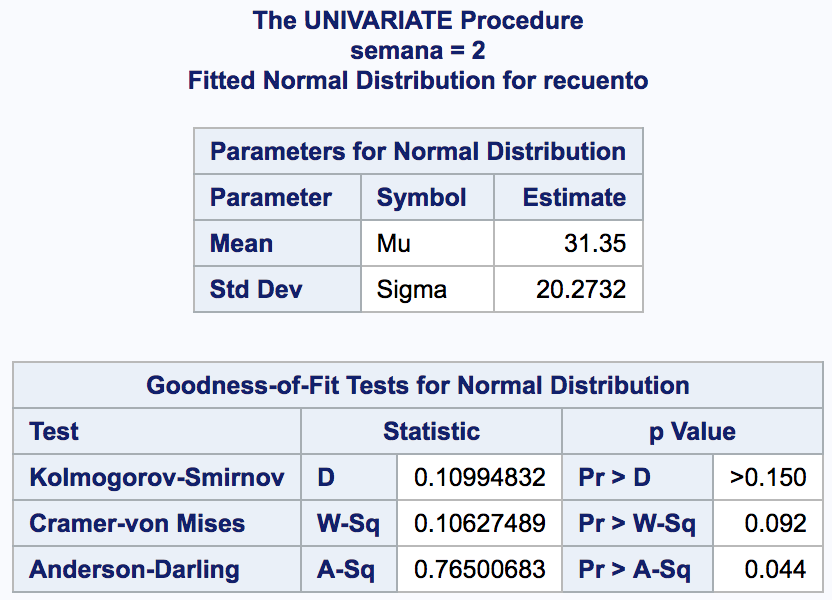
\includegraphics[width=\linewidth]{normality-2}
          \caption{}
          \label{fig:normality-2}
        \end{minipage}
        \begin{minipage}{.49\textwidth}
          \centering
          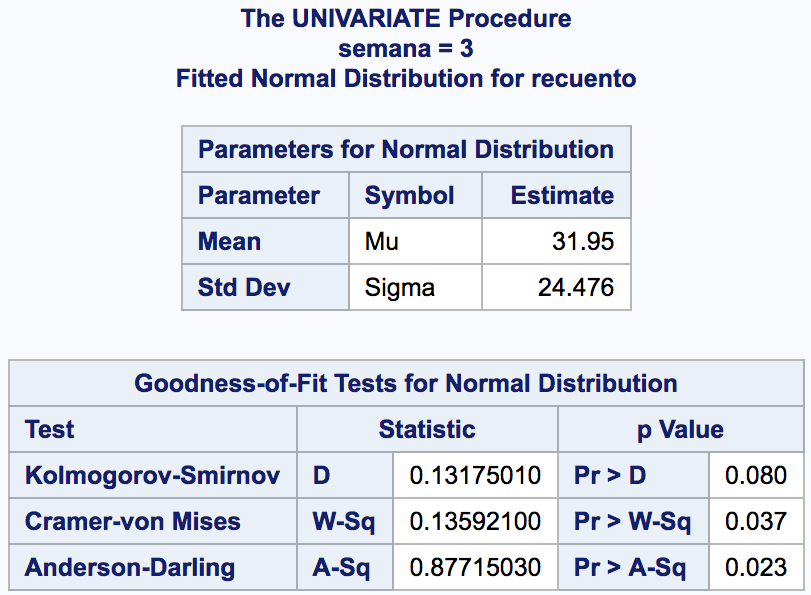
\includegraphics[width=\linewidth]{normality-3}
          \caption{}
          \label{fig:normality-3}
        \end{minipage}
        \begin{minipage}{.49\textwidth}
          \centering
          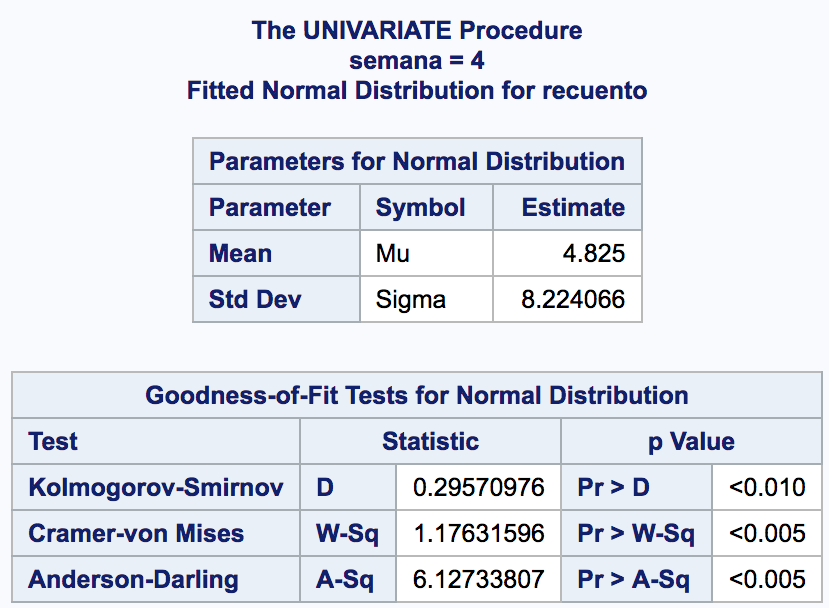
\includegraphics[width=\linewidth]{normality-4}
          \caption{}
          \label{fig:normality-4}
        \end{minipage}
        \begin{minipage}{.49\textwidth}
          \centering
          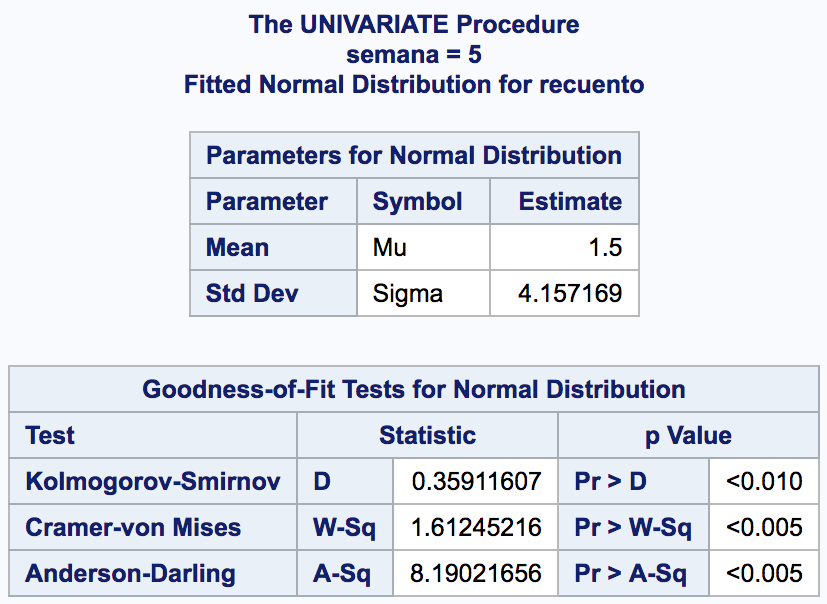
\includegraphics[width=\linewidth]{normality-5}
          \caption{}
          \label{fig:normality-5}
        \end{minipage}
        \begin{minipage}{.49\textwidth}
          \centering
          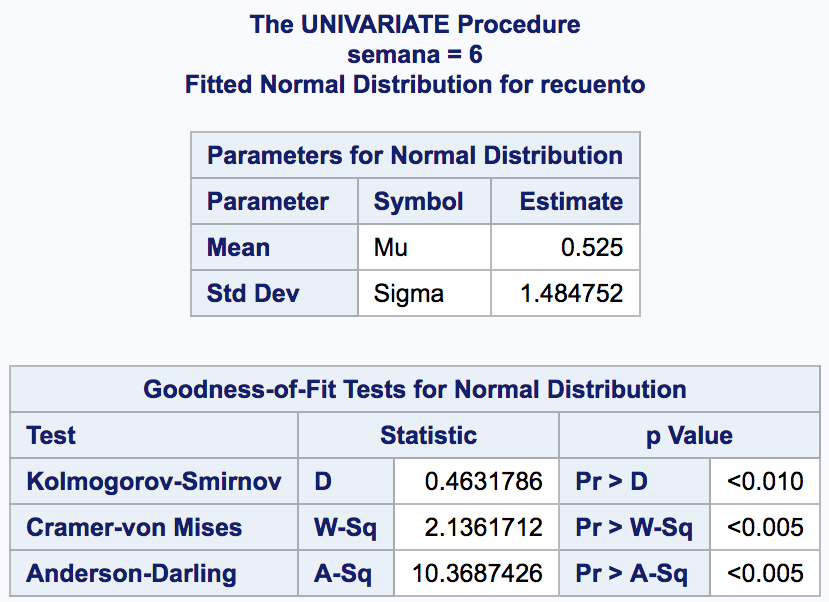
\includegraphics[width=\linewidth]{normality-6}
          \caption{}
          \label{fig:normality-6}
        \end{minipage}
      \end{figure}

      \begin{figure}
        \centering
        \begin{minipage}{.49\textwidth}
          \centering
          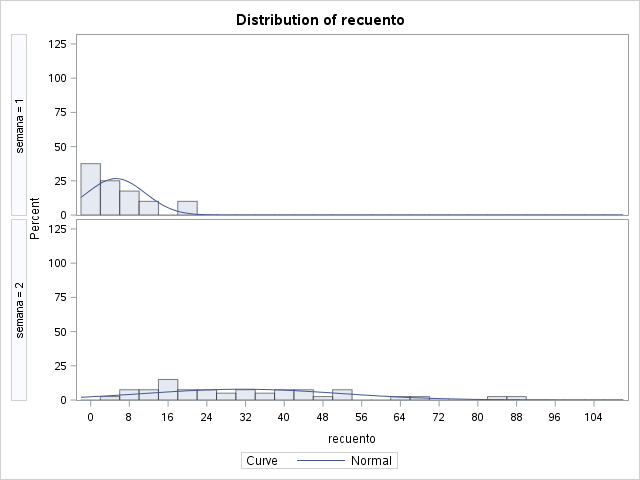
\includegraphics[width=\linewidth]{histogram-plot-1-2}
          \caption{Histograma: Semanas 1 y 2}
          \label{fig:histogram-plot-1-2}
        \end{minipage}
        \begin{minipage}{.49\textwidth}
          \centering
          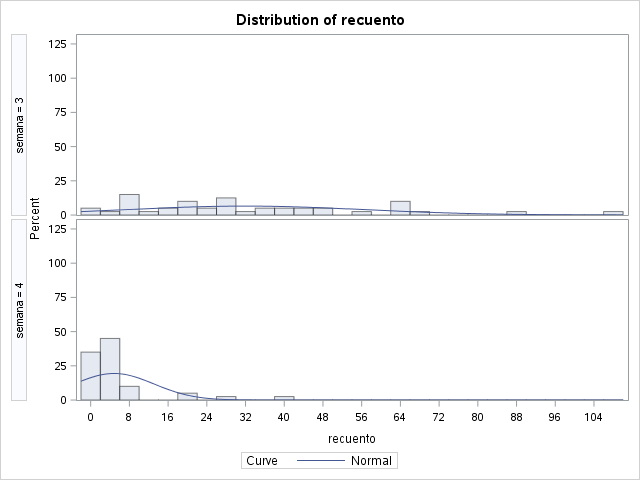
\includegraphics[width=\linewidth]{histogram-plot-3-4}
          \caption{Histograma: Semanas 3 y 4}
          \label{fig:histogram-plot-3-4}
        \end{minipage}
        \begin{minipage}{.49\textwidth}
          \centering
          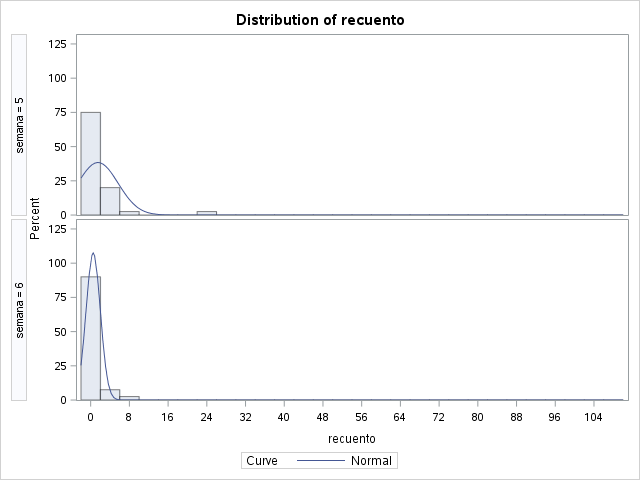
\includegraphics[width=\linewidth]{histogram-plot-5-6}
          \caption{Histograma: Semanas 5 y 6}
          \label{fig:histogram-plot-5-6}
        \end{minipage}
      \end{figure}

      \paragraph{}
      [TODO ]


      \begin{figure}
        \centering
        \begin{minipage}{.49\textwidth}
          \centering
          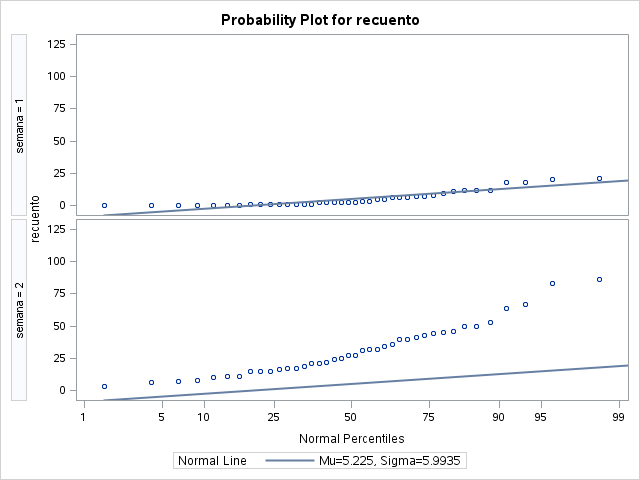
\includegraphics[width=\linewidth]{normal-plot-1-2}
          \caption{Gráfico de Normalidad: Semanas 1 y 2}
          \label{fig:normal-plot-1-2}
        \end{minipage}
        \begin{minipage}{.49\textwidth}
          \centering
          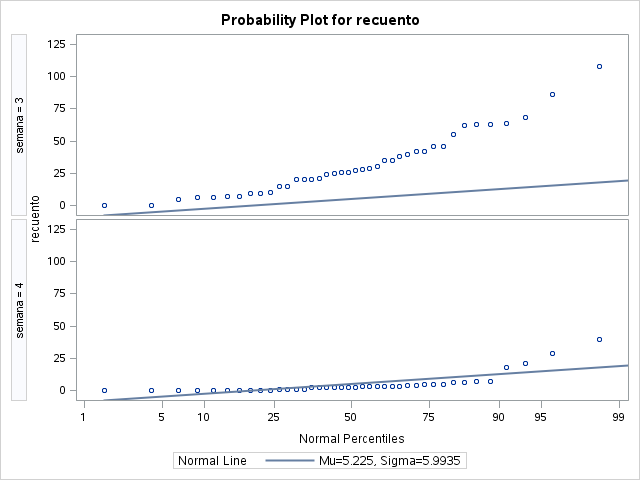
\includegraphics[width=\linewidth]{normal-plot-3-4}
          \caption{Gráfico de Normalidad: Semanas 3 y 4}
          \label{fig:normal-plot-3-4}
        \end{minipage}
        \begin{minipage}{.49\textwidth}
          \centering
          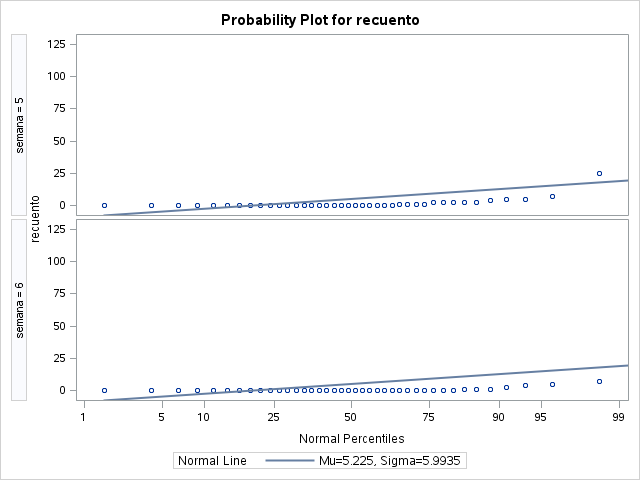
\includegraphics[width=\linewidth]{normal-plot-5-6}
          \caption{Gráfico de Normalidad: Semanas 5 y 6}
          \label{fig:normal-plot-5-6}
        \end{minipage}
      \end{figure}

    \subsection{Realiza el contraste de igualdad de medias y analiza los residuos. ?`Qué conclusiones sacas?}
    \label{sec:e2}

      \paragraph{}
      [TODO ]


    \subsection{Realiza el test de \emph{Levene}. ?`Te sorprende el resultado?}
    \label{sec:e3}

      \paragraph{}
      [TODO ]


    \subsection{Transforma la respuesta mediante $log(recuento + 1)$ y repite el apartado \ref{sec:e2}. ?`Qué cambios observas?}
    \label{sec:e4}

      \paragraph{}
      [TODO ]


    \subsection{Realiza el test de \emph{kruskal-Wallis} sobre los datos originales para contrastar la igualdad de medias}
    \label{sec:e5}
      \paragraph{}
      [TODO ]

  \section{Código fuente}
  \label{sec:code}

    \begin{figure}
      \centering
      \begin{minted}[frame=single,framesep=5pt]{sas}
data pulgones;
  do semana=1 to 6;
    do repet=1 to 40;
      input recuento @@;
      output;
    end;
  end;
  datalines;
  12 1 6 1 5 7 1 1 2 1 20 0 9 7 0 12 2 0 0 2 8 0 11 2 21 0 3 18 2 2 6 6
  5 1 12 0 3 1 1 18 40 16 32 15 44 41 43 53 67 21 6 31 15 11 21 40 15 50
  17 32 24 7 25 11 64 22 50 27 3 46 45 10 8 27 34 19 86 83 17 36 86 63
  20 68 55 42 24 29 20 27 26 63 40 46 7 15 10 30 46 26 15 42 6 28 7 9 5
  35 6 9 108 38 35 64 21 20 62 25 0 0 29 2 3 0 4 2 6 7 5 4 6 0 0 5 1 3 2
  2 2 5 0 1 1 0 3 1 2 0 3 3 18 7 21 0 0 0 2 3 0 40 5 7 0 0 0 1 1 2 1 0
  25 1 0 0 0 0 0 0 0 5 0 2 0 0 0 2 0 0 0 4 0 0 0 0 2 0 0 0 0 2 1 0 0 1 7
  0 0 0 4 1 5 2 0 0 0 0 0 0 0 0 0 0 0 0 0 0 0 0 0 0 0 0 0 0 0 0 0 0 0 0
;
run;
      \end{minted}
      \caption{\emph{Código SAS:} Lectura del conjunto de datos.}
      \label{code:sas_1}
    \end{figure}


    \begin{figure}
      \centering
      \begin{minted}[frame=single,framesep=5pt]{sas}
proc print data=pulgones (obs=5) n;
run;
      \end{minted}
      \caption{\emph{Código SAS:} Vista preliminar del conjunto de datos.}
      \label{code:sas_2}
    \end{figure}

    \begin{figure}
      \centering
      \begin{minted}[frame=single,framesep=5pt]{sas}
proc univariate data=pulgones;
   class semana;
   var recuento;
   probplot recuento / normal
                     (mu=est sigma=est color=blue w=1);
run;
      \end{minted}
      \caption{\emph{Código SAS:} Estudio Descriptivo de la variable \texttt{recuento} particionada por \texttt{semana}.}
      \label{code:sas_3}
    \end{figure}

    \begin{figure}
      \centering
      \begin{minted}[frame=single,framesep=5pt]{sas}
proc sgplot data=pulgones;
  vbox recuento /  group=semana;
run;
      \end{minted}
      \caption{\emph{Código SAS:} \emph{Box-Plot} de la variable \texttt{recuento} particionada por \texttt{semana}.}
      \label{code:sas_4}
    \end{figure}

    %-----------------------------
    %	Bibliographic references
    %-----------------------------

    \nocite{rano2017}

    \bibliographystyle{acm}
    \bibliography{bib}

\end{document}
